% !TeX root = ../../main.tex
\subsection{Continuous Execution and Grasp Preparation}
An episode initializes the simulator once. I first chooses whether to navigate
to the inspection pose; P then selects a permitted station or refuses. At
station arrival, calibrated depth backprojection and a gold-color RGB mask
localize the handle by fitting a vertical cylinder with known nominal radius.
G ranks the two grasp commands constructed from this estimate. Arm preparation
first tests a direct joint-space path, then uses a bounded RRT search
\citep{lavalle1998rrt} with 180 samples if needed. Position servos execute the
path before contact-based opening begins. Joint positions and velocities pass
continuously between stages, and each movement is followed by a real camera
observation. Figure~\ref{fig:active_motion} illustrates the inspection prefix
and the change in the reached view.
\ifshowfigures
% Recorded primary-policy example from test cohort C.
\begin{figure}[H]
  \centering
  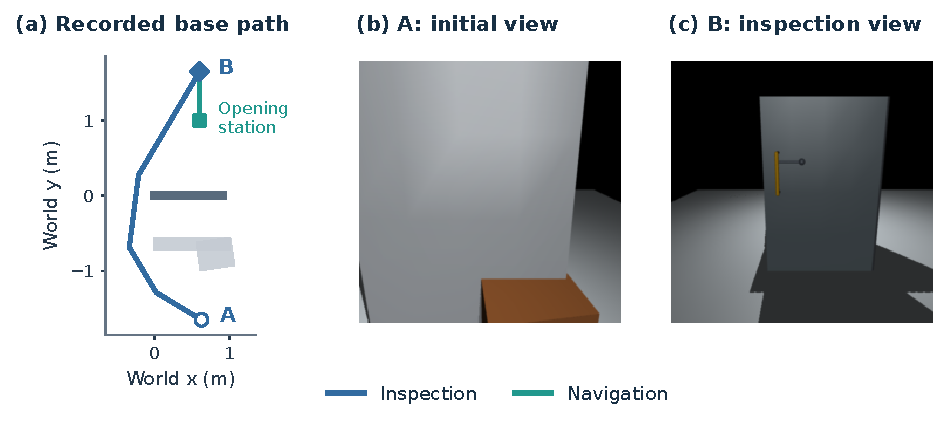
\includegraphics[width=\linewidth]{figures/methods/report_active_motion.pdf}
  \caption{Primary-policy replay from test cohort C. (a) Recorded base path with door and obstacle geometry in gray; viewpoints A and B correspond to (b) the initial view and (c) the reached inspection view. The base then reaches the opening station and opens the door. The episode covers 4.62~m in 61.99 simulated seconds.}
  \label{fig:active_motion}
\end{figure}

\fi
